\section{Funktionen}
Aus der Ist-Analyse und den eigenen Vorstellungen der neuen Plattform ergibt
sich ein Funktionsumfang, der im Prototyp umgesetzt werden soll. Diese
wiederum unterteile ich in `Muss' und `Kann' Funktionen. Erstere sollen
zwingend im Prototypen umgesetzt werden, die anderen behalte ich mir vor, je
nach noch zur Verfügung stehender Zeit umzusetzen oder nicht.

\subsection{Muss-Funktionen}
In der nachstehenden Tabelle \ref{tab:muss_funktionen} sind alle umzusetzenden 
Funktionen aufgelistet, nummeriert und näher beschrieben:

\begin{table}[h]
\begin{center}
    \begin{tabular}{llp{8cm}l}
        \toprule Nr & Funktion & Beschreibung \\
        \midrule 1 & Registrierung & Ein neuer Benutzer kann sich auf der Plattform
                     mit einem Benutzernamen und Passwort registrieren. \\
        \midrule 2 & Anmeldung & Ein registrierter Benutzer kann sich auf der
                     Plattform mit seinem Benutzernamen und Passwort anmelden. \\
        \midrule 3 & Filme verfassen & Filme können von Besuchern und angemeldeten Benutzern
                     betrachtet, erfasst, editiert und gelöscht werden. \\
        \midrule 4 & Bewertung sehen & Bewertungen können von Besuchern und angemeldeten Benutzern
                     betrachtet werden. \\
        \midrule 5 & Bewertung abgeben & Benutzer können eine Bewertung zu einem Film mit oder ohne
                     Kommentar abgeben. \\
        \midrule 6 & Bewertung Freundeskreis & Angemeldete Benutzer sehen zur normalen Bewertung zusätzlich
                     die Bewertung ihres Freundeskreises. \\
        \midrule 7 & Internationalisierung & Alle Inhalte können in deutscher und englischer
                     Sprache erfasst werden \\
        \midrule 8 & Schnittstelle & Die Funktionen 3 und 4 stehen ebenfalls in einer API 
                     zur Verfügung. \\
        \bottomrule
    \end{tabular}
    \caption{Zwingend umzusetzende Funktionen des Prototypen}
    \label{tab:muss_funktionen}
\end{center}
\end{table}

Anmerkung zur Funktion Nr. 7: Eine API (``Application-Programming-Interface''), auf 
Deutsch ``Programmierschnittstelle'', ist ein Programmteil, der von einem Softwaresystem 
anderen Programmen zur Anbindung an das System zur Verfügung gestellt wird \cite{api}.

Der Prototyp soll es anderen Programmen über diese Schnittstelle ermöglichen,
Filme und deren Bewertung abzurufen, zu erstellen, zu ändern und zu löschen.

\subsection{Kann-Funktionen}
In der nachstehenden Tabelle \ref{tab:kann_funktionen} sind alle optional 
umzusetzenden Funktionen aufgelistet, nummeriert und näher beschrieben.

Damit die `Muss' und `Kann' Funktionen nicht miteinander verwechselt werden 
können, wird die Nummerierung fortlaufend durchgeführt.

\begin{table}[h]
\begin{center}
    \begin{tabular}{llp{8cm}l}
        \toprule Nr & Funktion & Beschreibung \\
        \midrule 9 & Freunde verwalten & Angemeldete Benutzer können Freunde
                     zu ihrer Freundesliste hinzufügen und entfernen. \\
        \midrule 10 & Bewertungen verwalten & Angemeldete Benutzer können
                     in einer speziellen Ansicht alle ihre abgegebenen Bewertungen
                     und Kommentare zu Filmen bearbeiten und löschen. \\
        \midrule 11 & Favoritenliste & Angemeldete Benutzer können Filme ihrer
                     Favoritenliste hinzufügen und entfernen. \\
        \midrule 12 & Erweiterte Schnittstelle & Alle restlichen Funktionen
                     können ebenfalls, wenn nötig mit Authentifizierung, über
                     die API verwaltet werden. \\
        \bottomrule
    \end{tabular}
    \caption{Optional umzusetzende Funktionen des Prototypen}
    \label{tab:kann_funktionen}
\end{center}
\end{table}

\section{Ansichten}
Jene Funktionen, die für den Benutzer direkt abgebildet werden müssen, habe
ich in Wireframes \cite{wireframe} abgebildet, damit die eigentliche Umsetzung 
einfacher fällt.

\subsection{Grundlayout}
Als Basis einer Webapplikation dient ein gut durchdachtes Grundlayout, welches
Funktionen und Informationen, die jederzeit zur Verfügung stehen müssen, darstellt.
Wie zum Beispiel die Navigation, eine Registrier- und Anmeldefunktion und der Sprachwechsel.

In der Grafik \ref{01_grundlayout} ist ein Browserfenster abgebildet, das die
fiktive Adresse \url{http://oml.orwell.ch/} aufgerufen und geladen hat. Auf der Grafik
ist die Navigation mit drei fiktiven Menüpunkten, zwei zur Verfügung stehenden 
Sprachen und einem Registrierungs- und Anmeldebutton zu sehen. Auch ist klar erkennbar,
wo sich der Inhalt der jeweiligen Seiten befinden wird. Zusätzlich sieht man, welches
Menü und welche Sprache zur Zeit aktiv ist.

\begin{figure}[ht]
    \begin{center}
        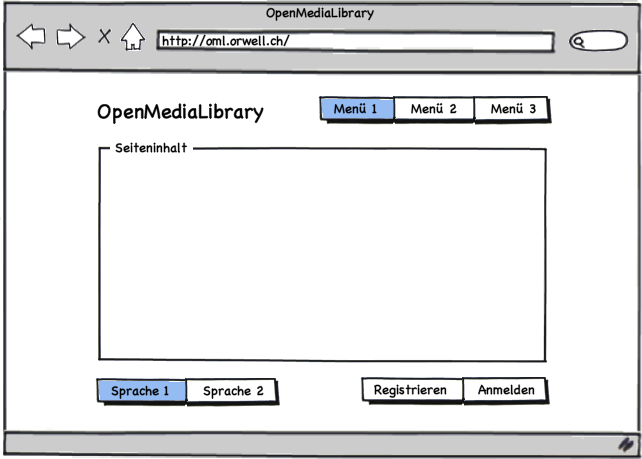
\includegraphics[width=1\textwidth,angle=0]{./wireframes/01_grundlayout.png}
        \caption{Wireframe des Grundlayouts}
        \label{01_grundlayout}
    \end{center}
\end{figure}

In den folgenden Ansichten wird jeweils der Seiteninhalt näher spezifiziert. Die
aktiven und inaktiven Menüs werden ebenfalls der aktuellen Seite angepasst.

\subsection{Registrierung}
In der Grafik \ref{02_registrierung} ist die Registrierung abgebildet. Um sich
auf der Plattform zu registrieren benötigt man einen Benutzername, der gleichzeitig
die E-Mailadresse des Benutzers ist. Hinzu kommt ein Passwort, dass man zur 
Bestätigung wiederholt eingeben muss.

\begin{figure}[ht]
    \begin{center}
        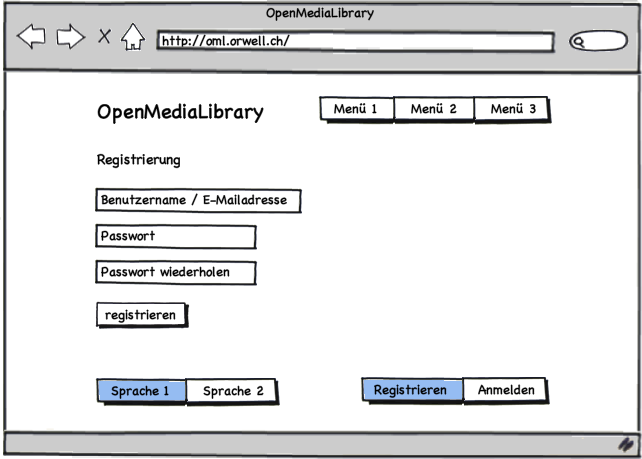
\includegraphics[width=1\textwidth,angle=0]{./wireframes/02_registrierung.png}
        \caption{Wireframe der Registrierung}
        \label{02_registrierung}
    \end{center}
\end{figure}

\clearpage

\subsection{Anmeldung}
Nachdem man sich erfolgreich registriert hat, kann man sich auf der Plattform
mit dem Benutzernamen und Passwort anmelden. Wie diese Anmeldung aussehen soll, sieht
man in der Grafik \ref{03_anmeldung}.

\begin{figure}[ht]
    \begin{center}
        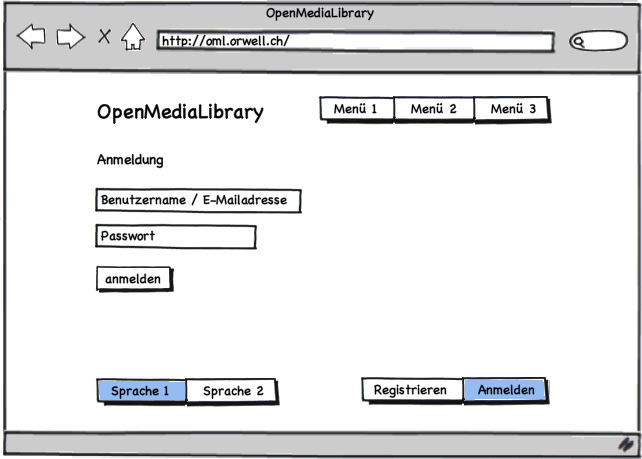
\includegraphics[width=1\textwidth,angle=0]{./wireframes/03_anmeldung.png}
        \caption{Wireframe der Anmeldung}
        \label{03_anmeldung}
    \end{center}
\end{figure}

\subsection{Filme}
Für die Darstellung der Filme gibt es vier verschiedene Ansichten:

\begin{enumerate}
    \item Übersicht und Auflistung aller vorhandenen Filme
    \item Detailansicht der Filme für Gäste und nicht angemeldete Benutzer
    \item Detailansicht der Filme für angemeldete Benutzer
    \item Bearbeitungsmaske des Filmes
\end{enumerate}

\subsubsection{1. Filmübersicht}
In der Grafik \ref{04_01_uebersicht} ist die erste Ansicht abgebildet. Es werden
alle vorhandenen Filme mit Namen aufgelistet. Zu jedem Film sind drei weiterführende
Funktionen verfügbar:

\begin{itemize}
    \item Details: Führt zur Detailansicht des Filmes
    \item Bearbeiten: Führt zur Bearbeitungsmaske des Filmes
    \item Löschen: Entfernt den Film von der Plattform
\end{itemize}

\begin{figure}[ht]
    \begin{center}
        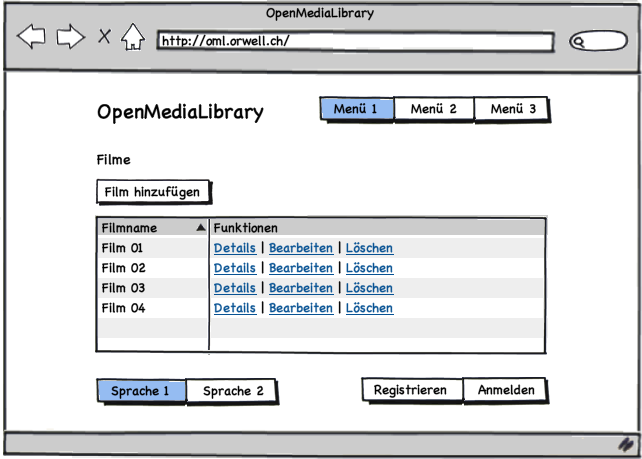
\includegraphics[width=1\textwidth,angle=0]{./wireframes/04_01_uebersicht.png}
        \caption{Wireframe der Filmübersicht}
        \label{04_01_uebersicht}
    \end{center}
\end{figure}

Zusätzlich zur Auflistung existiert ein Button zur Erstellung eines neuen Filmes.
Ich verzichte auf die Maske zur Erstellung eines neuen Filmes, da diese genau gleich
aussehen wird wie die Bearbeitungsmaske, jedoch ohne bestehendem Inhalt.

\subsubsection{2. Filmdetailansicht}
In der Grafik \ref{04_02_detail} sieht man die Detailansicht eines Filmes inklusive Bewertung
über alle Benutzer. Diese Angaben, wie auch die Filmübersicht, sind für Gäste und
unangemeldete Benutzer sichtbar.

\begin{figure}[ht]
    \begin{center}
        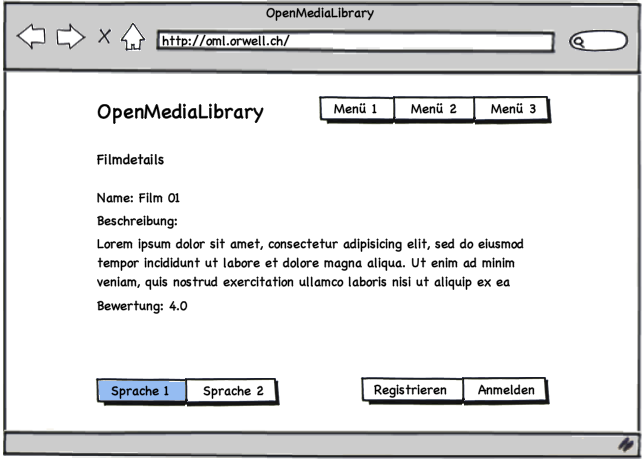
\includegraphics[width=1\textwidth,angle=0]{./wireframes/04_02_detail.png}
        \caption{Wireframe einer Filmdetailansicht für Gäste und nicht angemeldete Benutzer}
        \label{04_02_detail}
    \end{center}
\end{figure}

\clearpage

\subsubsection{3. Filmdetailansicht für angemeldete Benutzer}
Die zusätzlichen Funktionen wie die Maske zur Abgabe einer Bewertung und die Bewertungsangabe des Filmes 
seiner Freunde sehen nur angemeldete Benutzer und ist in der Grafik \ref{04_03_detail_angemeldet} 
ersichtlich. Die Maske um eine Bewertung abzugeben ist zudem nur zu sehen, sofern der angemeldete
Benutzer noch keine Bewertung abgegeben hat. In diesem Falle sieht der Benutzer an dieser
Stelle seine eigene Bewertung und kann diese bearbeiten oder entfernen.

\begin{figure}[ht]
    \begin{center}
        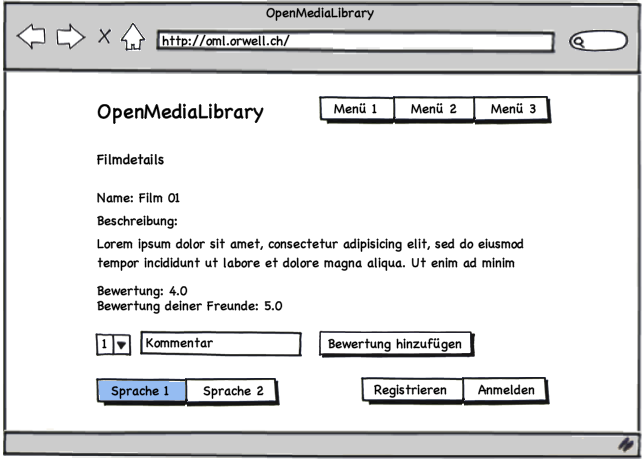
\includegraphics[width=1\textwidth,angle=0]{./wireframes/04_03_detail_angemeldet.png}
        \caption{Wireframe einer Filmdetailansicht für angemeldete Benutzer}
        \label{04_03_detail_angemeldet}
    \end{center}
\end{figure}

\subsubsection{4. Bearbeitungsmaske eines Filmes}
In dieser Ansicht kann man den Namen und die Beschreibung des Filmes bearbeiten.
Wie diese aussehen soll, sieht man in der Grafik \ref{04_04_edit}.

\begin{figure}[ht]
    \begin{center}
        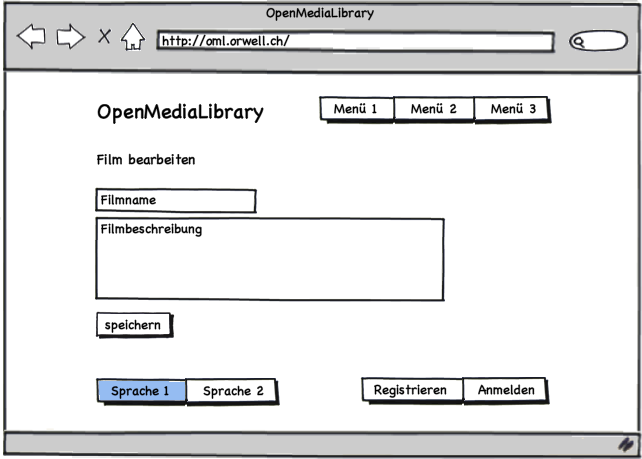
\includegraphics[width=1\textwidth,angle=0]{./wireframes/04_04_edit.png}
        \caption{Wireframe der Bearbeitungsmaske eines Filmes}
        \label{04_04_edit}
    \end{center}
\end{figure}

\clearpage

\section{Entity Relationship Model}
Aufgrund der definierten Funktionen und den Wireframes kann jetzt ein ER-Modell
erstellt werden. In der Grafik \ref{erm} ist das vollständige Modell des Prototypen
abgebildet.

Die Namen der Objekte sind in Englisch, da der Quellcode ausschliesslich in englischer 
Sprache geschrieben und kommentiert wird. Dies habe ich mit Absicht gewählt, 
damit es später für Drittentwickler keine unnötige Sprachbarriere gibt.

\begin{figure}[ht]
    \begin{center}
        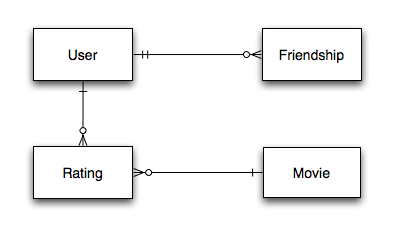
\includegraphics[width=0.6\textwidth,angle=0]{./erm/erm.png}
        \caption{ER-Modell des Prototypen}
        \label{erm}
    \end{center}
\end{figure}

In der Tabelle \ref{tab:erm} gehe ich auf die einzelnen Objekte des Modells ein
und erläutere ihre Funktion im Protoyp.

\begin{table}[ht]
\begin{center}
    \begin{tabular}{llp{10cm}l}
        \toprule Nr & Name & Funktion \\
        \midrule 1 & User & Bildet einen Benutzer im System ab. Ein Benutzer
                     kann keine bis mehrere Freunde (``Friendship'') haben. \\
        \midrule 2 & Friendship & Bildet eine Freundschaft zwischen genau zwei
                     Benutzern im System ab. Zu einer akzeptierten Freundschaft 
                     gehören immer genau zwei Benutzer. \\
        \midrule 3 & Rating & Bildet eine Bewertung eines Filmes, eines Benutzers
                     im System ab. Ein Benutzer kann mehrere Filme bewerten und
                     somit keine bis mehrere Bewertungen haben und eine 
                     existierende Bewertung gehört immer genau zu einem Benutzer 
                     und einem Film (``Movie''). \\
        \midrule 4 & Movie & Bildet einen Film im System ab. Ein Film kann keine
                     oder mehrere Bewertungen erhalten. \\
        \bottomrule
    \end{tabular}
    \caption{Erläuterungen zu den Objekten im ER-Modell}
    \label{tab:erm}
\end{center}
\end{table}

\clearpage

\section{Objektattribute}
Die Objekte im System haben genau definierte Attribute. Gewisse Attribute sind
statisch zum Objekt abgelegt, andere werden dynamisch berechnet. Da dies einen
Einfluss auf die Programmierung des Prototypen hat, werden diese explizit 
unterschieden.

In der Tabelle \ref{tab:attribute} liste ich alle Attribute
der einzelnen Objekte auf, beschreibe ihre Funktion und kennzeichne sie mit
einem `S' für statisch und einem `D' für dynamisch. Die Namen der Attribute sind 
ebenfalls ausschliesslich in englischer Sprache.

\begin{table}[ht]
\begin{center}
    \begin{tabular}{lllcp{9cm}l}
        \toprule Nr & Objekt & Attribut & Art & Funktion \\
        \midrule
            1 & User & Username & S & Beinhaltet den Benutzernamen des Benutzer. \\
            & & Password & S & Beinhaltet das Passwort des Benutzers. \\
            & & Ratings & D & Gibt alle Bewertungen des Benutzers zurück. \\
            & & Pending Friends & D & Gibt alle Freunde zurück, wo die Freundschaftsanfragen
                                      des Benutzers noch offen sind. \\
            & & Direct Friends & D & Gibt alle Freunde zurück, wo die Freundschaftsanfragen
                                     des Benutzers bereits akzeptiert wurden. \\
            & & Inverse Friends & D & Gibt alle Freunde zurück, wo die Freundschaftsanfragen,
                                      die an den Benutzer gestellt worden sind, vom Benutzer
                                      akzeptiert wurden. \\
            & & Friends & D & Gibt alle Freunde, wo die Freundschaftsanfragen akzeptiert wurden,
                              egal ob die Freundschaftsanfrage direkt oder indirekt gestellt
                              wurden, zurück. \\
        \midrule
            2 & Friendship & User & S & Beinhaltet den Benutzer, der die Freundschaftsanfrage
                                        gestellt hat. \\
            & & Friend & S & Beinhaltet den Benutzer, an den die Freundschaftsanfrage gestellt
                                        wurde. \\
            & & Approved & S & Beinhaltet, ob die Freundschaftsanfrage akzeptiert wurde oder nicht. \\
        \midrule
            3 & Rating & User & S & Beinhaltet den Benutzer, der die Bewertung erfasst hat. \\
            & & Movie & S & Beinhaltet den Film, der bewertet wurde. \\
            & & Value & S & Beinhaltet die eigentliche Bewertung, also eine ganze Zahl zwischen 1 und 10. \\
            & & Comment & S & Beinhaltet optional zur Bewertung einen Kommentar des Benutzers. \\
        \midrule
            4 & Movie & Title & S & Beinhaltet den Namen des Filmes. \\
            & & Description & S & Beinhaltet die Beschreibung des Filmes. \\
            & & Ratings & D & Gibt alle Bewertungen des Filmes zurück. \\
            & & Users & D & Gibt alle Benutzer zurück, die den Film bewertet haben. \\
            & & Rating All & D & Gibt den Mittelwert über alle Bewertungen aller Benutzer zurück. \\
            & & Rating Friends & D & Gibt den Mittelwert über alle Bewertungen der Freunde des 
                                 angemeldeten Benutzers zurück. \\
        \bottomrule
    \end{tabular}
    \caption{Erläuterungen zu den statischen und dynamischen Attributen der Objekte}
    \label{tab:attribute}
\end{center}
\end{table}
